% !TEX root = main.tex
%%%%%%%%%%%%%%%%%%%%%%%%%%%%%%%%%%%%%%%%%%%%%%%%%%%%%%%%%%%%%%%%%%%%%%%%%%%%%%%%
% Time Between Failures Analysis
%%%%%%%%%%%%%%%%%%%%%%%%%%%%%%%%%%%%%%%%%%%%%%%%%%%%%%%%%%%%%%%%%%%%%%%%%%%%%%%%
\section{Time Between Failures Analysis}
\label{section:tbf}

\begin{figure}[bt]
  \begin{center}
    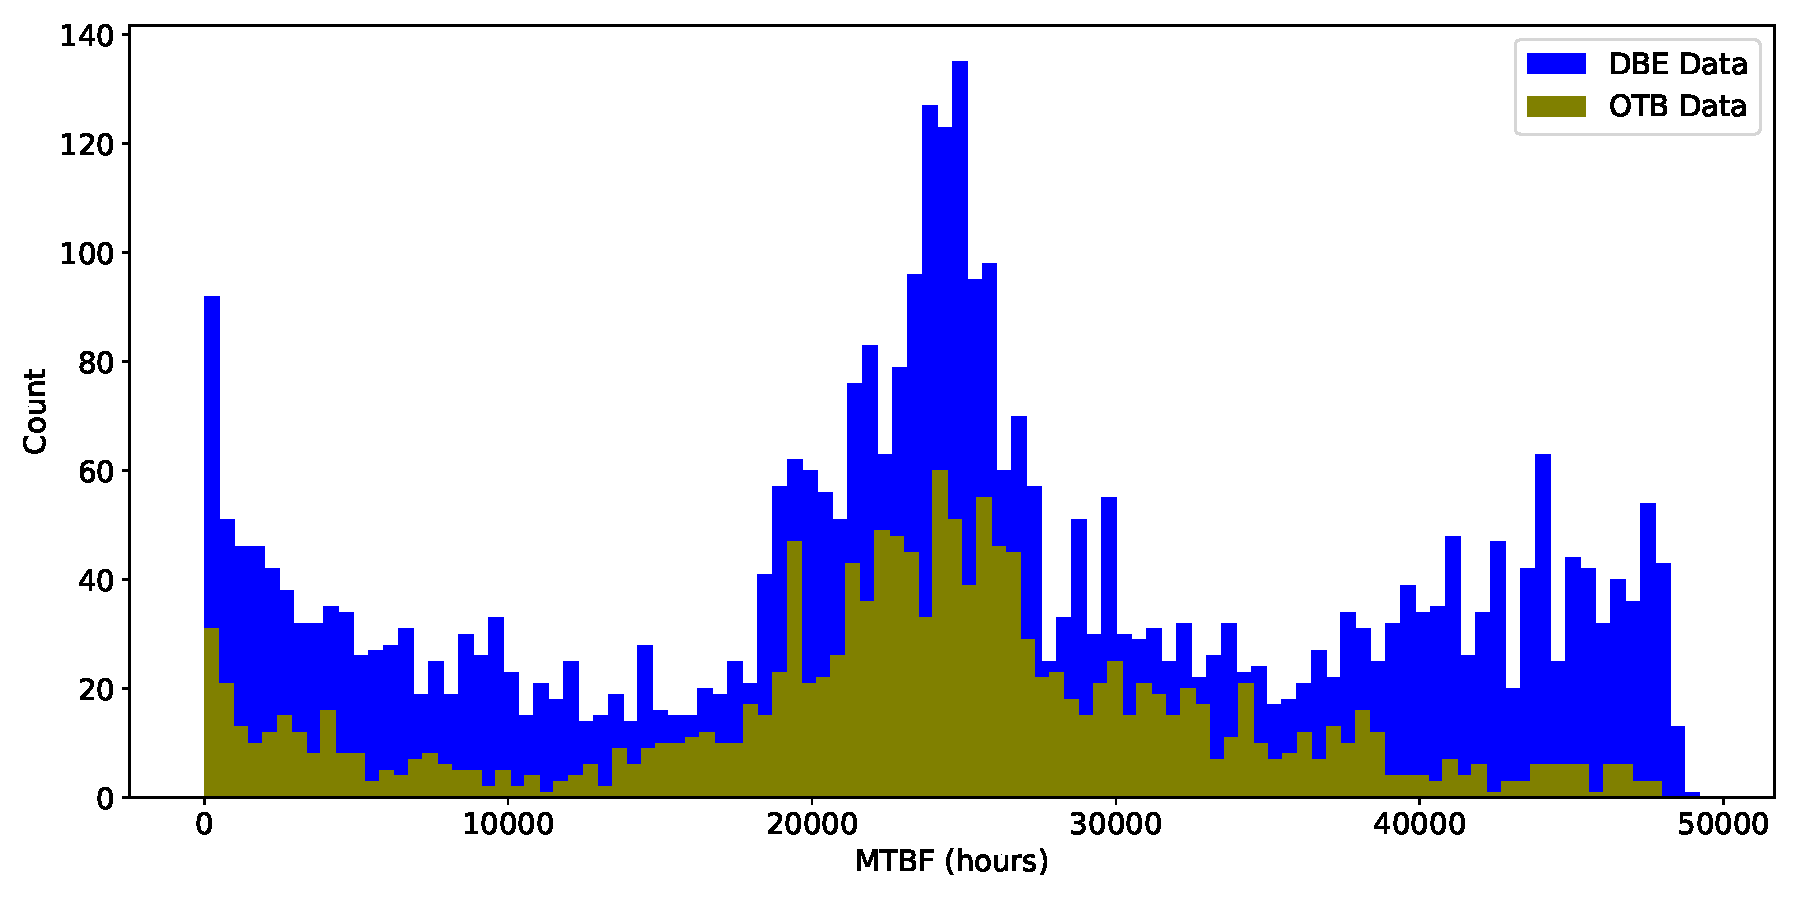
\includegraphics[width=\columnwidth]{figs/MTBF_GPUwise.pdf}
  \end{center}
  \caption{Distribution of MTBFs due to DBEs and OTBs across all GPUs.}
  \label{fig:Device_MTBFs}
\end{figure}

Using the processed data, we analyze the inter-arrival times between the DBE and OTB events. 
This analysis is done at the device level and the system level. 
It provides important insights into the reliability of large-scale machines, where the 
failure rate of an individual device is significantly different from the overall reliability
of the machine.  

A histogram of MTBFs measured across GPUs which had at least one failure event is shown 
in Figure~\ref{fig:Device_MTBFs}. This is a practical assessment of device reliabilities 
as opposed to those provided in the device datasheet. The failures are tracked using the
SN of the GPUs even though a GPU might have been placed at different locations in the 
machine during its lifetime. The time to the first failure on a device is measured by taking
the insert time as the reference point, whereas, a simple difference is taken for subsequent
failures. It can be noticed that MTBFs due to DBE and OTB failures of most GPUs are clustered around 
25,000 hours or 2.8 years. Apart from the center cluster, a significant portion of GPUs has a very 
low MTBF (less than 1.5 hours) due to both DBE and OTB failures. This shows that a device 
can see a failure immediately after it is put into service or multiple events are caused due 
to a single root cause. On the other end of the spectrum, a noticeable portion of GPUs have very high
MTBFs due to DBE failures. This indicates that most GPUs see a single DBE during their lifetime.
Apart from this behavior, the distribution of MTBF due to DBE events looks very similar to that due 
to OTB events. Overall, it can be noted from Figure~\ref{fig:Device_MTBFs} that the number of recorded 
DBE events is significantly higher than the OTB events. 

%\begin{figure}[bt]
%  \begin{center}
%    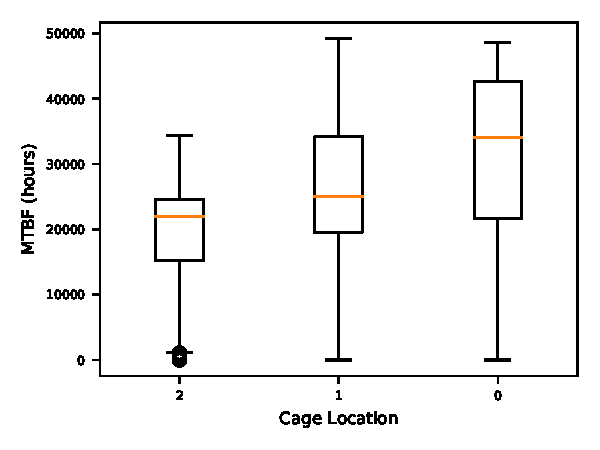
\includegraphics[width=\columnwidth]{figs/MTBF_CageWise.pdf}
%  \end{center}
%  \caption{MTBFs due to either DBEs or OTBs across the GPUs located in different cages.}
%  \label{fig:CageWise_MTBFs}
%\end{figure}

%\fix{Figure~\ref{fig:CageWise_MTBFs} shows temperature effect clearly. Should we move this 
%result to later in the paper?}

\begin{figure}[bt]
  \begin{center}
    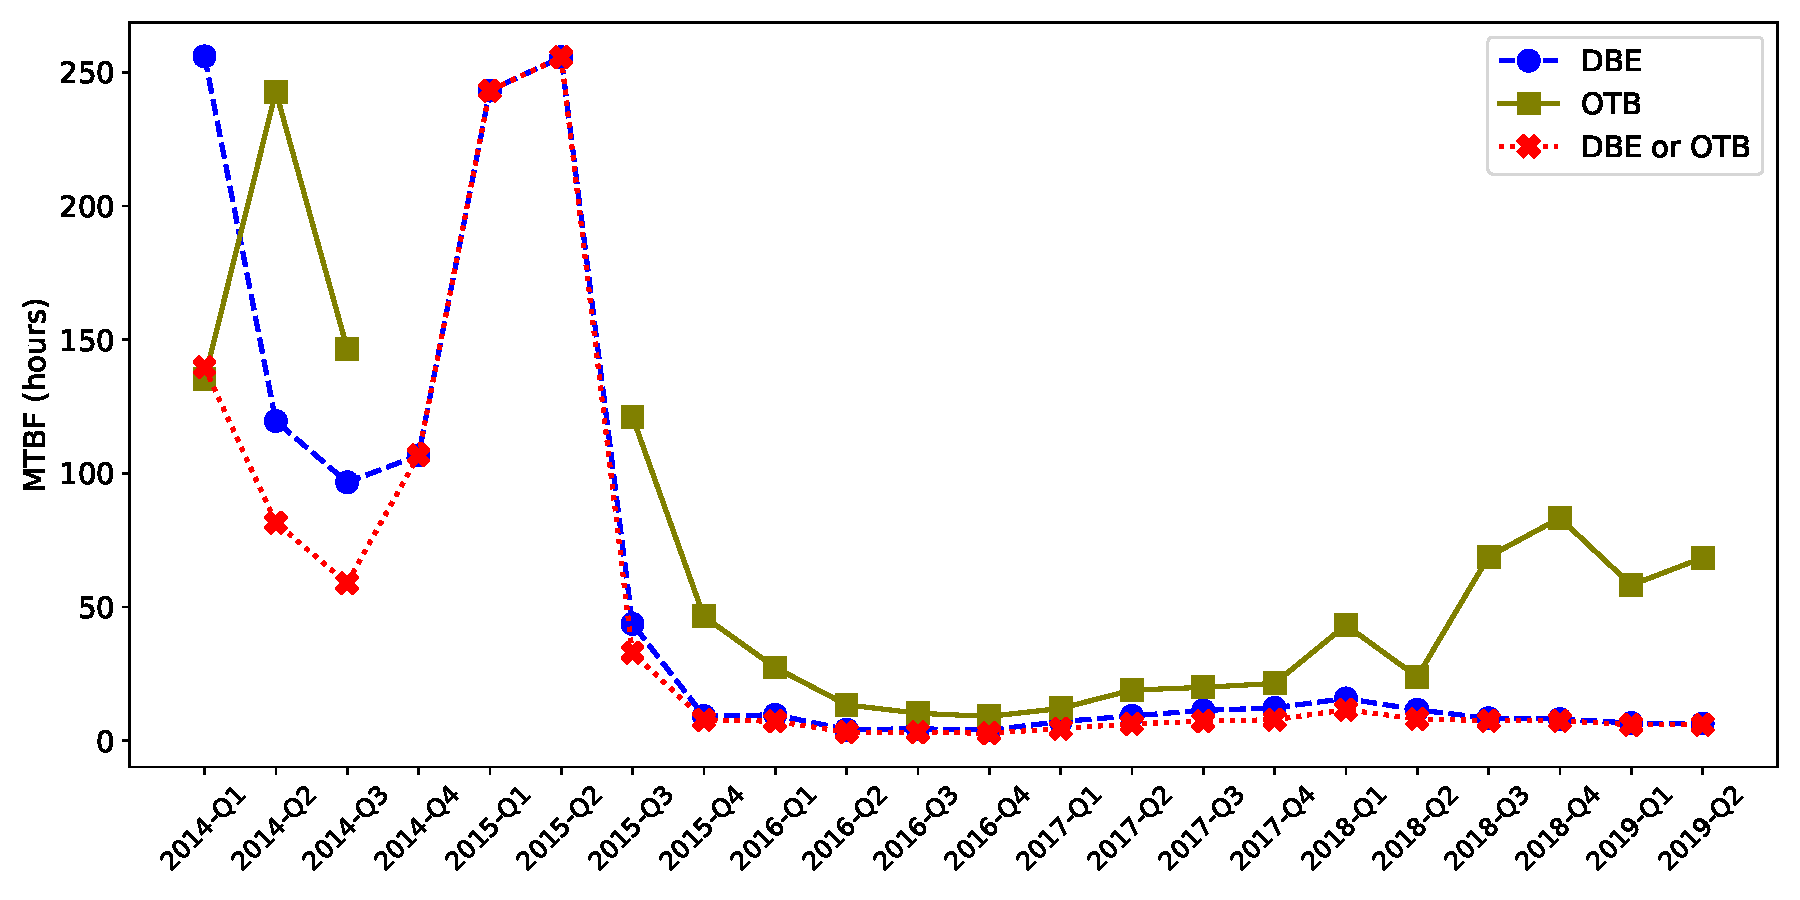
\includegraphics[width=\columnwidth]{figs/MTBF_quaterly_sys.pdf}
  \end{center}
  \caption{Variation of system-wide MTBF over the lifetime of the machine (time is segmented into quarters, 
i.e., January through March is Q1, so on).}
  \label{fig:MTBF_sys}
\end{figure}

\begin{figure}[bt]
  \begin{center}
    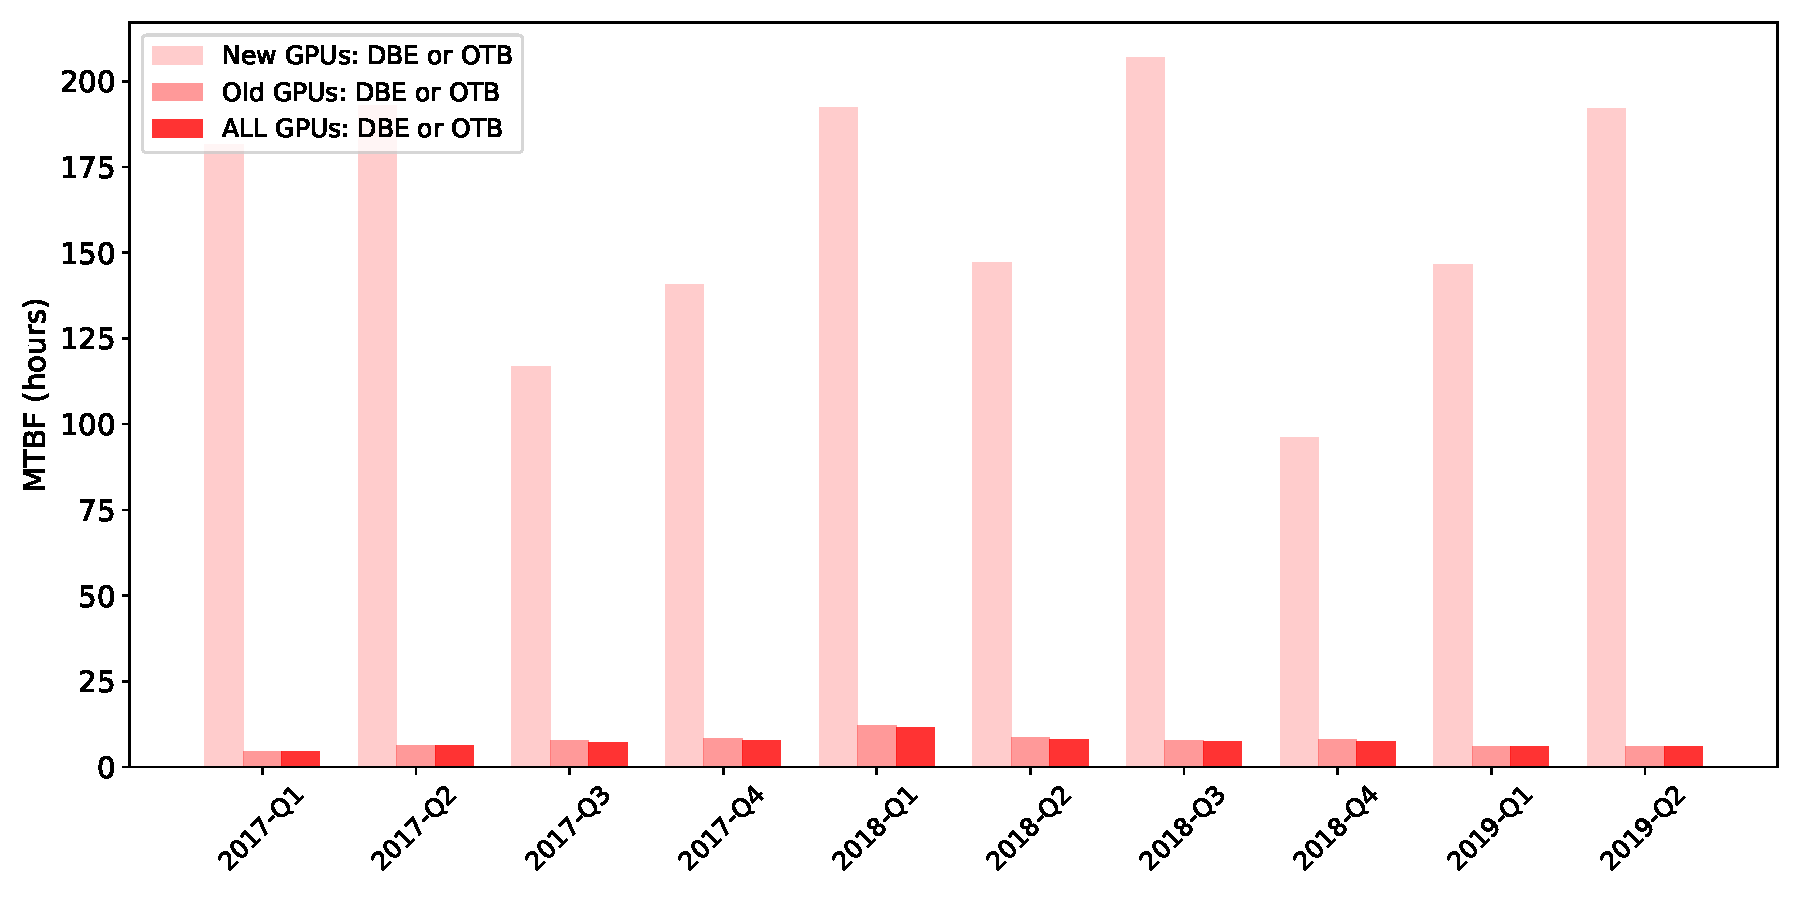
\includegraphics[width=\columnwidth]{figs/MTBF_quaterly_sys_NewOldALL.pdf}
  \end{center}
  \caption{Variation of system-wide MTBF across hypothetical new and old partitions of the machine over time.}
  \label{fig:MTBF_sys_NewOld}
\end{figure}

Although individual device MTBFs provide important insights into the varying failure rates
observed across the machine. It is worthwhile to perform a system-wide MTBF analysis since 
most high-performance computing applications use a significant number of GPUs in parallel. 
In the following analysis, failures occurring across all GPUs are consolidated and time between failures
is calculated. The old and new GPUs are all considered. At any given time, only a fixed number of GPUs
are in operation so any variation in time-between-failures is due to individual device reliabilities.

That said, a single MTBF number does not give an accurate picture of this machine.
With many GPU relocations and replacements across the machine over its lifetime, it is 
best to consider the variation of MTBF across fixed periods. Herein, we calculate 
the mean of time-between-failures across three months. Figure~\ref{fig:MTBF_sys}
clearly shows the considerable change in system-wide MTBF from one period to another. 
The observation of the MTBF trend shows the different phases which the machine went through. 
For example, when considering failure due to both DBE and OTB events more than 4X drop in MTBF is 
noted from 2015-Q3 to 2015-Q4 (note, MTBF of earlier quarters was significantly higher and is not 
included in the figure to better visualize various change points). This period marked the start of 
a rapid decline in system-wide MTBF until 2016-Q4. The rapid rise in the number of failures before this 
quarter can be seen in Figure~\ref{fig:NumFails_sys}. When GPU replacements start to take place in late 
2016, it triggers an increase in MTBF. However, this change only lasts until 2018-Q1, when we see another 
downward trend of system MTBF. Incidentally, 2018-Q1 also marks the completion of all GPU replacements. 
So the upward trend noted in the period from 2016-Q4 to 2018-Q1 might be attributed to a portion of the machine 
being unavailable while the reworks were taking place. A single replacement cycle lasted multiple weeks. 
%\fix{need to verify how long the replacement took}
There is no definite way to incorporate this unavailability of the machine into MTBF analysis, so it has to
be said that overall there has been an increase in MTBF of the machine due to the replacements. 
For example, before 2017-Q1, a MTBF as low as 2.7 hours is noted, whereas the lowest MTBF is 5.9 hours after this 
period. With such huge variations in system MTBF, it is difficult to reliably run applications even while using 
failure recovery approaches such as checkpoint restart, as discussed later on in Section~\ref{section:discussion}. 

The mean-time-between DBE and OTB failures are also separately tracked in this analysis.
One observation is the drastic increase in mean-time-between OTB failures after the GPU replacements.
This is also evident from the reduction of the absolute number of OTB failures in Figure~\ref{fig:NumFails_sys}.
However, the system MTBF is determined by the weakest link and the occurrence of DBE events tends to dictate it.
Even though the replacements helped to increase the MTBF due to DBE events by a factor, the overall system 
reliability is dictated by the components with the most age in the system. There is a re-emergence of upward trend towards 
the end of life in the number of DBE failures in Figure~\ref{fig:NumFails_sys} which almost all of them are due to 
older GPUs in the system. 

To better understand the difference in reliability of newer and old portions of the machine, 
Figure~\ref{fig:MTBF_sys_NewOld} shows the drastic difference in system MTBF measured in two hypothetical
partitions of the machine starting from the time when the majority of GPU replacements have been completed. 
The new partition of the machine has always 12X better MTBF than the older partition
of the machine. For example, in 2018-Q4, the MTBF recorded across old partition is about 7.9 hours, whereas it is about
96 hours (4 days) for the newer partition. The implications of such a huge disparity on applications running on the 
system are discussed in Section~\ref{section:discussion}. The insignificant difference in MTBF measured across all GPUs and
old partition of the machine can also be noted in Figure~\ref{fig:MTBF_sys_NewOld}.  
Therefore, the old GPUs that occupy a minority portion of the machine after GPU replacements, 
and have a disproportionately high number of failures and contribute towards a low system MTBF play a major role 
in determining the overall reliability of the machine.
The next section quantifies the survivability of this machine with its varied MTBF characteristics beyond its operational lifetime.
\fix{George, can you please check the last sentence, where I make a connection with the next section.}

\begin{figure}[bt]
  \begin{center}
    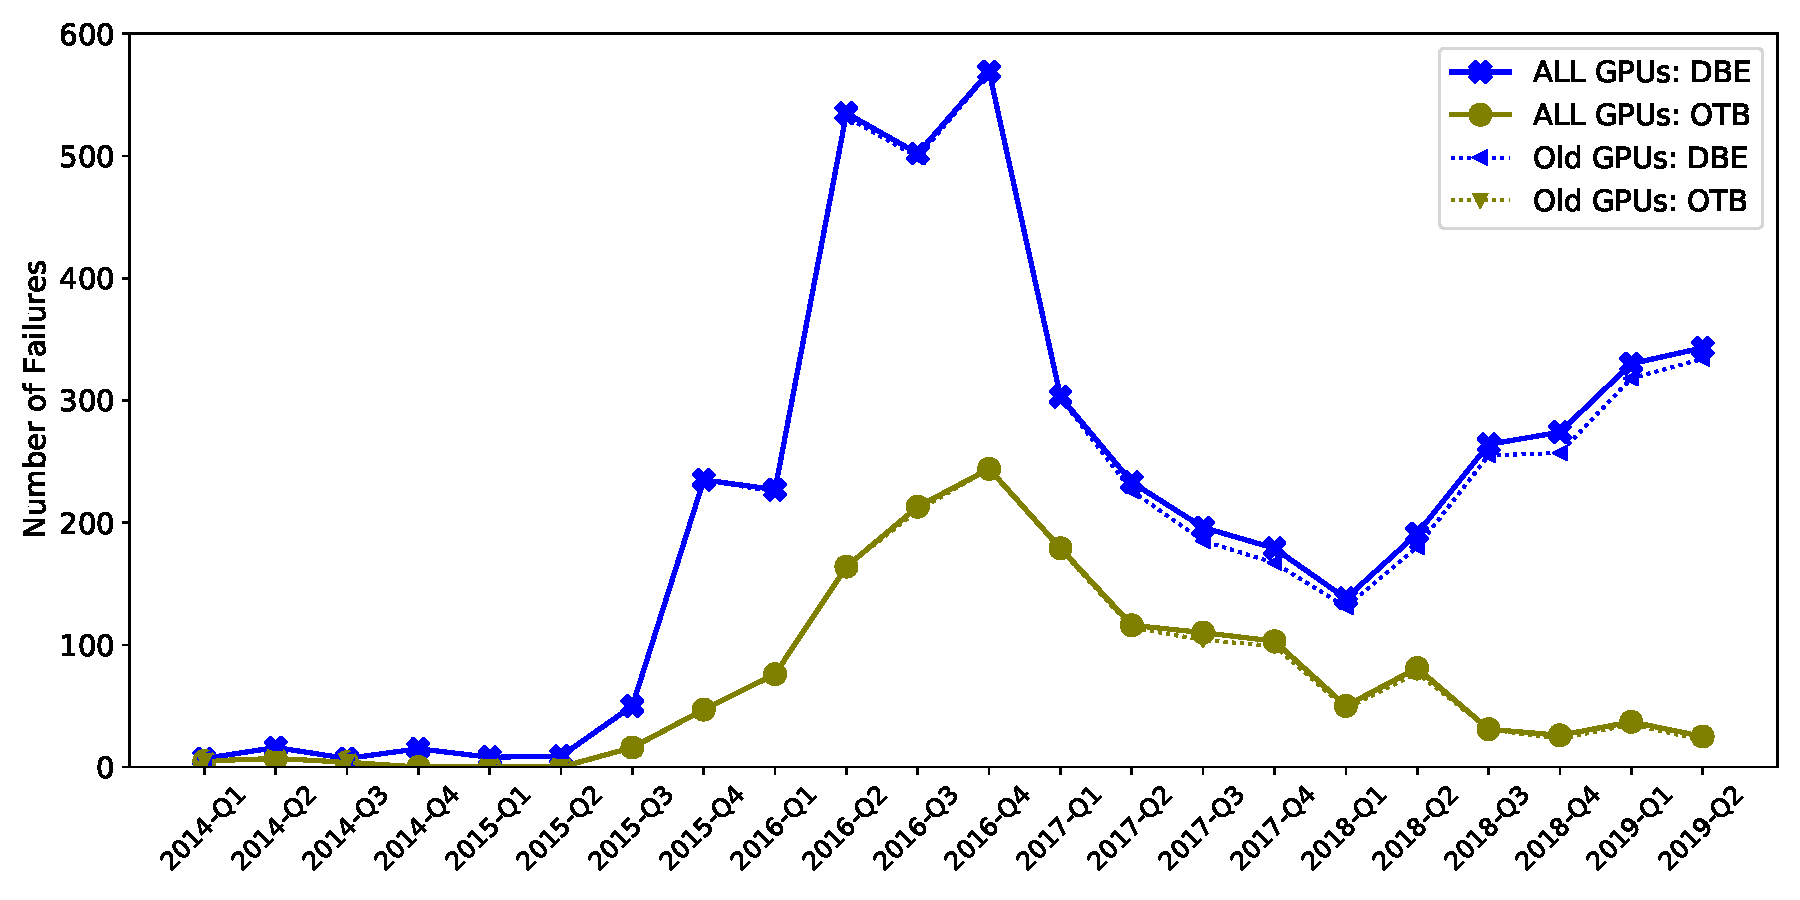
\includegraphics[width=\columnwidth]{figs/NumFailures_Quarterly_newOld.pdf}
  \end{center}
  \caption{The number of DBE and OTB failures observed over the lifetime of the machine.
A distinction is made for GPU failures happening across old GPUs to highlight the number 
of failures across the newer GPUs.}
  \label{fig:NumFails_sys}
\end{figure}
